La interfaz principal de RoboSim se ve de esta manera: 

\begin{figure}[H]
    \centering
    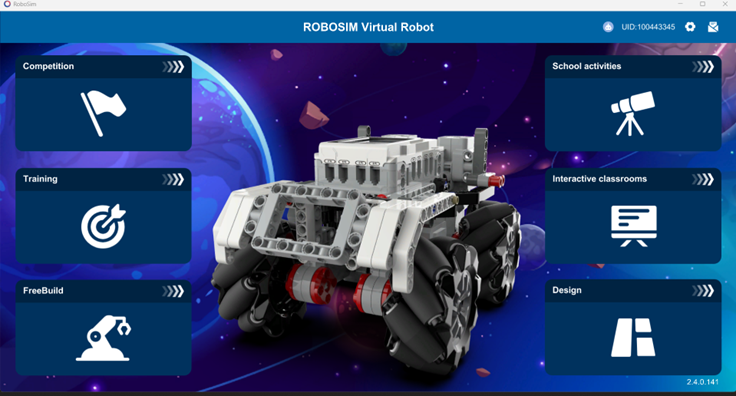
\includegraphics[scale = 0.70]{Imagenes/interfaz1.png}
    \caption{Interfaz principal del software}{Fuente: Propia}
\end{figure}

En donde podemos apreciar las diferentes opciones que nos ofrece este software de simulación

\textbf{Competencia en línea:} Muestra las competencias disponibles. Al hacer clic en una competencia específica, podrás ver el registro y acceder al lugar del evento.

\textbf{Entrenamiento temático:} Ofrece espacios de práctica basados en distintos temas de competencia.

\textbf{Construcción libre:} Permite construir el robot sin restricciones y guardar los archivos de construcción en tu computadora.

\textbf{Recursos del curso:} Diseñados para adaptarse a los materiales utilizados en RoboSim.

\textbf{Diseño de lugares:} Crea y edita espacios de entrenamiento de manera independiente.
